\documentclass[dvipsnames,10pt]{beamer}
\usetheme{m}
\metroset{block=fill,progressbar=frametitle}
\usepackage{fontspec}
\usepackage{graphicx,overpic}
\usepackage{hyperref}
\usepackage{xcolor}

\usepackage{microtype}

\usepackage{textcomp}                       % fix warning with missing font shapes
\usepackage{xspace}                         % to get the right spacing after macros
\usepackage{polyglossia}
\setdefaultlanguage{french}                   % indent the first paragraph of each section
\usepackage[font=small]{quoting}            % text citations

\usepackage{amsmath,amssymb,amsthm,amsfonts}% math
\usepackage{dsfont}
\usepackage{array}
\usepackage{booktabs}
\usepackage{algorithm}
\usepackage{algpseudocode}
\usepackage[autostyle=true,
            french=guillemets]{csquotes}   % automates some stylistic choices language-dependent: using \mkbibquote command you will get caporali quotes (i.e. « »)

\usepackage[style=philosophy-modern,
            hyperref,backref,natbib,
            backend=biber]{biblatex}
\bibliography{../bibliography}

\usepackage{forest}
\usepackage{pgfplots}
\pgfplotsset{compat=1.12}
\usetikzlibrary{arrows,3d}
\usepackage{float}
\usepackage[list=on]{subcaption}

\usefonttheme{dailyplanet}

\usepackage[scaled=1.1]{newtxsf}

\uselanguage{french}
\languagepath{french}
\deftranslation[to=french]{Theorem}{Théorème}
\deftranslation[to=french]{Lemma}{Lemme}
\deftranslation[to=french]{definition}{Définition}

\pgfplotsset{yticklabel style={text width=3em,align=right}}
\pgfplotsset{grid style={solid,black}}
\pgfplotsset{minor grid style={dashed,black}}

\makeatletter
\renewcommand{\ALG@name}{Algorithme}
\makeatother
\renewcommand{\algorithmicend}{\textbf{fin}}
\renewcommand{\algorithmicdo}{\textbf{faire}}
\renewcommand{\algorithmicwhile}{\textbf{tant que}}
\renewcommand{\algorithmicfor}{\textbf{pour}}
\renewcommand{\algorithmicreturn}{\textbf{renvoyer}}
\renewcommand{\algorithmicif}{\textbf{si}}
\renewcommand{\algorithmicthen}{\textbf{alors}}
\renewcommand{\algorithmicelse}{\textbf{sinon}}

%\setmainfont{Minion Pro}

\newcommand{\sgn}{\operatorname{sgn}}
\newcommand{\conv}{\operatorname{conv}}
\newcommand{\vect}{\operatorname{vect}}
\DeclareMathOperator*{\argmin}{arg\,min}
\DeclareMathOperator*{\argmax}{arg\,max}
\newcommand*\diff{\mathop{}\!\mathrm{d}}
\newcommand{\Var}{\mathrm{Var}}

\theoremstyle{plain}
\newtheorem{prop}{Proposition}
\newtheorem{theoreme}{Théorème}
\newtheorem{lemme}{Lemme}
\newtheorem{corol}{Corollaire}
\theoremstyle{definition}
\newtheorem{ex}[section]{Exemple}

\title{Ensembles d'arbres}
\subtitle{Théorie et application au scoring}
\author{Guillaume Ausset - Paris Saclay}
\institute{M2 MASEF - Crédit Agricole GRO}
\date{30 novembre 2016}
\frenchspacing

\begin{document}
\addtobeamertemplate{block begin}{\setlength\abovedisplayskip{0pt}}

\begin{frame}
    \titlepage
\end{frame}

\plain{Introduction}

\begin{frame}
\frametitle{Plan}
    \vspace{0.2cm}
    \tableofcontents
\end{frame}

\section{Rappels théoriques sur l'apprentissage}
\subsection{Scoring et mesure des performances}

\begin{frame}
\frametitle{La classification binaire}
\textbf{Classification binaire:} étant donné $\mathbf{x}_i \in \mathcal{X}$, déterminer $y_i \in \mathcal{Y} = \left\{0,1\right\}$
\begin{align*}
    \mathrm{Err} &= \frac{\mathrm{FP}+\mathrm{FN}}{\mathrm{TP}+\mathrm{FN}+\mathrm{FP}+\mathrm{TN}} \\
    \mathrm{Err}_\mathrm{équilibrée} &= \beta \frac{\mathrm{FP}}{\mathrm{TN}+\mathrm{FP}} + (1-\beta) \frac{\mathrm{FN}}{\mathrm{TP}+\mathrm{FN}} \\
    \mathrm{G-mesure} &= \sqrt{\frac{\mathrm{FP}}{\mathrm{TN}+\mathrm{FP}} * \frac{\mathrm{FN}}{\mathrm{TP}+\mathrm{FN}}} \\
    \mathrm{Precision} &= \frac{\mathrm{TP}}{\mathrm{TP} + \mathrm{FP}} \\
    \mathrm{Recall} &= \frac{\mathrm{TP}}{\mathrm{TP} + \mathrm{FN}} \\
    \mathrm{F-mesure} &= \frac{2 \times \mathrm{Precision} \times \mathrm{Recall}}{\mathrm{Precision} + \mathrm{Recall}}
\end{align*}
\emph{Problème:} mesures pas adaptées à la problématique du scoring.
\end{frame}

\begin{frame}
\frametitle{Scoring}
\textbf{Score:} classification binaire à l'aide d'une variable latente sur laquelle la classification en elle-même pourra se faire par analyse discriminante.
    \begin{equation*}
        \begin{cases}
            y = 1 \text{ si } S(x) \geq s \\
            y = 0 \text{ si } S(x) < s
        \end{cases}
    \end{equation*}
On veut que le score soit \emph{bien ordonné}:
\begin{equation}
    S(x_1) > S(x_2) \Leftrightarrow \mathbb{P} \left( y_1 = 1 \mid x_1 \right) > \mathbb{P} \left( y_2 = 1 \mid x_2 \right)
    \label{equ:score.ordoné}
\end{equation}
et (si possible) \emph{bien calibré}:
\begin{equation*}
    S(x) = \mathbb{P} \left( y = 1 \mid x \right)
    \label{equ:score.calibré}
\end{equation*}
\end{frame}

\begin{frame}
\frametitle{Mesure de performance pour le scoring: AUC}
Si l'on note $t$ le seuil de décision et $T$ la sortie de notre classifieur, on a
\begin{equation*}
    \mathbb{P} ( T > t \mid Y = 1 ) \simeq \frac{\mathrm{TP} (t) }{\mathrm{TP} (t) +\mathrm{FN} (t) } 
\end{equation*}
et de la même façon
\begin{equation*}
    \mathbb{P} ( T > t \mid Y = 0 ) \simeq \frac{\mathrm{FP} (t)}{\mathrm{TN} (t) +\mathrm{FP} (t)}
\end{equation*}
La courbe ROC est alors la courbe paramétrée:
\begin{equation*}
    \mathrm{ROC} (t) = \begin{bmatrix}
        \mathbb{P} ( T > t \mid Y = 0 ) \\
        \mathbb{P} ( T > t \mid Y = 1 )
    \end{bmatrix}
\end{equation*}
Sous cette forme l'AUC se calcule comme:
\begin{align*}
    \mathrm{AUC} &=  - \int_0^1 \mathbb{P} ( T > t \mid Y = 1 ) \mathbb{P}' ( T > t \mid Y = 0 ) \diff t \\
    &= \int_0^1 \mathbb{P} ( T > t \mid Y = 1 ) p ( t \mid Y = 0 ) \diff t
\end{align*}
\end{frame}

\begin{frame}
\frametitle{Mesures de performances: AUC}
\begin{figure}[htbp]
\centering
    \begin{tikzpicture}
    \begin{axis}[domain=0:1, ymin=0, ymax = 1, enlargelimits = false, xlabel = {Taux de faux positifs}, ylabel = {Taux de vrais positifs}, legend style={draw=none}]
            \addplot[no markers, const plot, mLightBrown, fill=mLightBrown!10] table [x = "fpr", y = "tpr", col sep = comma] {../images/roc_rf.csv} \closedcycle ;
            \node[mLightBrown] at (axis cs:0.8,0.1) {$\mathrm{AUC} = 0.805$};
            \addplot[no markers, black, dashed] {x}
                [yshift=8pt] node[pos=0.5,rotate=40] {\tiny{Modèle aléatoire}} ;
            \addplot[no markers, black, dashed] {x}
                [yshift=-8pt] node[pos=0.54,rotate=40] {\tiny{$\mathrm{AUC} = 0.5$}};
    \end{axis}
    \end{tikzpicture}
    \caption{Courbe ROC et AUC.}
\end{figure}
\end{frame}

\begin{frame}
\frametitle{Mesures de performances: AUC}
On obtient alors une interprétation de l'AUC qui explique tout son intérêt dans le cas du scoring:
\begin{align*}
    \mathbb{P} ( T^i > T^j \mid Y^i = 1 , Y^j = 0 ) &= \iint_{ \{ (t^i,t^j) : t^i > t^j) \} } p(t^i,t^j \mid Y^i = 1 , Y^j = 0 ) \diff t^i \diff t^j \\
    &= \int_0^1 \left( \int_{t^j}^1 p(t^i \mid Y^i = 1 ) \diff t^i  \right) p(t^j \mid Y^j = 0 ) \diff t^j \\
    &= \int_0^1 \mathbb{P} ( T > t^j \mid Y = 1 ) p(t^j \mid Y^j = 0 ) \diff t^j \\
    &= \mathrm{AUC}
\end{align*}
\end{frame}

\begin{frame}
\frametitle{Mesures de performances: règles de scoring propres}
\begin{definition}[Régle de scoring propre]
    Une règle de scoring
    \begin{equation*}
        R : [0,1]^J \times \mathcal{Y} \rightarrow \mathbb{R}
    \end{equation*}
    est dite propre si et seulement si
    \begin{equation*}
        \left( \mathbb{P}(c_1),\dotsc,\mathbb{P}(c_J)\right) = \argmax_p \mathbb{E}_Y \left[ R(p,y) \right]
    \end{equation*}
\end{definition}
\begin{description}
    \item[\textbf{Règle logarithmique}] \begin{equation*}
        R(p,y) = \log ( p_{i_y} )
    \end{equation*}
    \item[\textbf{Règle quadratique de Brier}] \begin{equation*}
        R(p,y) = 2 p_{i_y} - \Vert p \Vert_2
    \end{equation*}
    \item[\textbf{Règle sphérique}] \begin{equation*}
        R(p,y) = \frac{p_{i_y}}{\Vert p \Vert_2}
    \end{equation*}
\end{description}
où $i_y$ est l'indice de la classe de $y$.
\end{frame}

\subsection{Théorie de Vapnik-Chervonenkis}

\begin{frame}
\frametitle{Minimisation du risque empirique}
Problème d'approximation de $f$ par une famille de fonctions, mais $f$ connue seulement en certains points. On remplace la distance entre les fonctions par la \emph{perte} aux points $(\mathbf{x}_i,y_i)$:
\begin{equation*}
    L(\varphi_{\mathcal{L}} (y_i,\mathbf{x}_i))
\end{equation*}
On minimise la perte moyenne
\begin{align*}
    \mathrm{Err} \left( \varphi  \right) &= \mathbb{E}_{X,Y} \left[ L(\varphi_{\mathcal{L}} (Y,\mathcal{X})) \right] \\
    \varphi^\star &= \argmin_{\varphi_{\mathcal{L}} \in \Phi} \mathbb{E}_{X,Y} \left[ L\left(Y,\varphi_{\mathcal{L}}\left(X\right)\right) \right] \\
    &\simeq \argmin_{\varphi_{\mathcal{L}} \in \Phi} \frac{1}{N} \sum_{i=1}^N L\left(y_i,\varphi_{\mathcal{L}}\left(\mathbf{x}_i\right)\right) \\
    \mathrm{Err}_N \left( \varphi_{\mathcal{L}} \right) &= \frac{1}{N} \sum_{i=1}^N L\left(y_i,\varphi_{\mathcal{L}}\left(\mathbf{x}_i\right)\right) \\
    \varphi_{\mathcal{L}}^\star &= \argmin_{\varphi \in \Phi} \mathrm{Err}_N \left( \varphi  \right)
\end{align*}
\end{frame}

\begin{frame}
\frametitle{Consistence}
\begin{definition}
    La procédure ERM est consistante si:
    \begin{align*}
        \mathrm{Err} \left( \varphi_{\mathcal{L}}^\star \right) \xrightarrow[\vert \mathcal{L} \vert \to +\infty]{\mathbb{P}} \mathrm{Err} ( \varphi^\star ) \\
        \mathrm{Err}_N \left( \varphi_{\mathcal{L}}^\star \right) \xrightarrow[\vert \mathcal{L} \vert \to +\infty]{\mathbb{P}} \mathrm{Err} ( \varphi^\star )
    \end{align*}
\end{definition}
\begin{theoreme}[Théorème fondamental de l'apprentissage]
    Pour une fonction de perte $L$ bornée, la méthode ERM est consistante si et seulement si le risque empirique converge uniformément vers le vrai risque, c'est-à-dire:
    \begin{equation}
        \lim_{\vert \mathcal{L} \vert \to +\infty} \mathbb{P} \left( \sup_{\varphi \in \Phi} \vert \mathrm{Err} ( \varphi_{\mathcal{L}} ) - \mathrm{Err}_N ( \varphi_{\mathcal{L}} ) \vert > \varepsilon \right) = 0 \label{equ:vc.consistant}
    \end{equation}
\end{theoreme}
\end{frame}

\begin{frame}
\frametitle{VC dans le cas de la classification}
\begin{theoreme}\label{thrm:vc}
    Dans le cas de la classification binaire et avec la perte $0/1$ on a:
    \begin{align}
        &\mathbb{P} \left( \sup_{\varphi \in \Phi} \vert \mathrm{Err}_N ( \varphi ) - \mathrm{Err} ( \varphi ) \vert > \varepsilon \right) \leq 8 G(\Phi,N) e^{-N \varepsilon^2 / 32} \\
        &\mathbb{E} \left[ \sup_{\varphi \in \Phi} \vert \mathrm{Err}_N ( \varphi ) - \mathrm{Err} ( \varphi ) \vert \right] \leq 2 \sqrt{\frac{\log G(\Phi,N) + \log 2 }{N}}
    \end{align}
\end{theoreme}
Or,
\begin{equation*}
    G(\Phi,N) \leq h \left( 1 + \ln \left( \frac{N}{h} \right) \right)
\end{equation*}
Donc il suffit de contrôler $h$, la dimension de VC. \\
\textbf{Conclusion:} Les méthodes introduites plus tard seront consistantes.
\end{frame}

\section{Méthodes ensemblistes}
\subsection{Décomposition biais-variance}

\begin{frame}
\frametitle{Biais-variance: cas de la régression}
\begin{theoreme}[Décomposition biais-variance, \cite{Geman1992}]
    Dans le cas de la perte $L^2$ on a:
    \begin{equation}
        \mathbb{E}_{\mathcal{L}} \left[ \operatorname{Err} ( \varphi_{\mathcal{L}} (x) ) \right] = \operatorname{bruit} (x) + \operatorname{biais}^2 (x) + \operatorname{var} (x)
    \end{equation}
    où
    \begin{align*}
        \operatorname{bruit} (x) &= \operatorname{Err} (\varphi_{B} (x) ) \\
        \operatorname{biais}^2 (x) &= ( \varphi_B (x) - \mathbb{E}_{\mathcal{L}} \left[ \varphi_{\mathcal{L}} (x) \right] )^2 \\
        \operatorname{var} (x) &= \mathbb{E}_{\mathcal{L}} \left[ \left( \varphi_{\mathcal{L}} (x) - \mathbb{E}_{\mathcal{L}} [ \varphi_{\mathcal{L}} (x) ] \right)^2 \right]
    \end{align*}
    ( Rappel: $\mathrm{Err}\left(\varphi_{\mathcal{L}}\right) = \mathbb{E}_{X,Y} \left[ L \left(Y,\varphi_{\mathcal{L}} \left(X \right) \right) \right]$ )
\end{theoreme}
\end{frame}

\begin{frame}
\frametitle{Biais-variance: dilemme}
\begin{figure}[H]
    \centering
    \begin{tikzpicture}
    \begin{axis}[%
    name=plot1,width=0.5\textwidth,
      height=0.4\textwidth,
    domain=0:2*pi, ymin=-1.2, ymax = 1.2]
    \addplot[no markers, smooth] {sin(deg(x))};
            \foreach \yindex in {2,...,21}
                \addplot[no markers, smooth, mLightBrown, thick, opacity = 0.1] table [x index = 1, y index = \yindex, col sep = comma] {../images/model1.csv};
    \end{axis}

    \begin{axis}[%
    name=plot2,width=0.5\textwidth,
      height=0.4\textwidth,
    at=(plot1.right of south east), anchor=left of south west,
    domain=0:2*pi, ymin=-1.2, ymax = 1.2]
    \addplot[no markers, smooth] {sin(deg(x))};
            \foreach \yindex in {2,...,21}
                \addplot[no markers, smooth, mLightBrown, thick, opacity = 0.1] table [x index = 1, y index = \yindex, col sep = comma] {../images/model3.csv};
    \end{axis}

    \begin{axis}[%
    name=plot4,width=0.5\textwidth,
      height=0.4\textwidth,
    at=(plot2.below south west), anchor=above north west,
    domain=0:2*pi, ymin=-1.2, ymax = 1.2]
    \addplot[no markers, smooth] {sin(deg(x))};
            \foreach \yindex in {2,...,21}
                \addplot[no markers, smooth, mLightBrown, thick, opacity = 0.1] table [x index = 1, y index = \yindex, col sep = comma] {../images/model20.csv};
    \end{axis}

    \begin{axis}[%
    name=plot3,width=0.5\textwidth,
      height=0.4\textwidth,
    at=(plot4.left of south west), anchor=right of south east,
    domain=0:2*pi, ymin=-1.2, ymax = 1.2]
    \addplot[no markers, smooth] {sin(deg(x))};
            \foreach \yindex in {2,...,21}
                \addplot[no markers, smooth, mLightBrown, thick, opacity = 0.1] table [x index = 1, y index = \yindex, col sep = comma] {../images/model5.csv};
    \end{axis}
    \end{tikzpicture}
    \caption{Apprentissage de $\sin (x)$ sur $[0,2 \pi]$ à l'aide de polynômes de degrés $1$,$3$,$5$ et $20$.}\label{fig:biaisvar}
\end{figure}
\end{frame}

\begin{frame}
\frametitle{Biais-variance: cas de la perte 0-1}
Sous la règle de décision: $\varphi_{\mathcal{L}} (x) = \argmax_{c \in \mathcal{Y}} \hat{p}_\mathcal{L} ( Y = c \mid X = x )$, on trouve la décomposition:
\begin{align*}
    &\mathbb{E}_{\mathcal{L}} \left[ \mathbb{E}_{Y \mid X = x} \left[ \mathds{1}_{\varphi_{\mathcal{L}} (x) \neq Y } \right]  \right] \\
    &= \mathbb{P} \left( \varphi_B (x) \neq Y \right) + \mathbb{P}_{\mathcal{L}} \left( \varphi_{\mathcal{L}} (x) \neq \varphi_B (x) \right) \left( 2 \mathbb{P} \left( \varphi_B (x) = Y \right) - 1 \right)
\end{align*}
Si l'on suppose alors que $\hat{p}_{\mathcal{L}} (Y = \varphi_B (x)) \sim \mathcal{N}$:\begin{theoreme}[\cite{Louppe2014}]
Pour la perte 0-1 dans le cas de la classification, l'erreur de généralisation attendue $\mathbb{E}_{\mathcal{L}} \left[ \operatorname{Err} ( \varphi_{\mathcal{L}} (x) ) \right]$ en $ X = x $ admet la décomposition suivante:
\begin{align*}
    &\mathbb{E}_{\mathcal{L}} \left[ \operatorname{Err} ( \varphi_{\mathcal{L}} (x) ) \right] = \mathbb{P} ( \varphi_B (x) \neq Y ) + \dotsb \\
    &\dotsb + \Phi \left( \frac{0.5 - \mathbb{E}_{\mathcal{L}} [ \hat{p}_{\mathcal{L}} (Y = \varphi_B (x)) ] }{\sqrt{\mathbb{V}_{\mathcal{L}} \hat{p}_{\mathcal{L}} (Y = \varphi_B (x)) } } \right) \left( 2 \mathbb{P} ( \varphi_B (x) = Y ) - 1 \right)
\end{align*}
\end{theoreme}
\end{frame}

\subsection{Moyennage de classifieurs}

\begin{frame}
\frametitle{Réduction de la variance par moyennage}
\begin{theoreme}[\cite{Louppe2014}, cas de la régression $L^2$]
\begin{equation*}
    \psi_{\mathcal{L},1,\dotsc,M} (x) = \frac{1}{M} \sum_{m=1}^M \varphi_{\mathcal{L},m} (x)  
\end{equation*}
        
\begin{equation*}
    \mathbb{E}_{\mathcal{L}} \left[ \operatorname{Err}(\psi_{\mathcal{L},1,\dotsc,M} (x)) \right] = \mathrm{bruit}(x) + \mathrm{biais}^2 (x) + \mathrm{var} (x)
\end{equation*}
\begin{align*}
    \mathrm{bruit}(x) &= \operatorname{Err} ( \varphi_B (x) ) \\
    \mathrm{biais}^2 (x) &= \left( \varphi_B (x) - \mathbb{E}_{\mathcal{L},i} \left[ \varphi_{\mathcal{L},i} (x) \right] \right)^2 \\
    \mathrm{var} (x) &= \rho (x) \sigma^2_{\mathcal{L},i} (x) + \frac{1-\rho (x)}{M} \sigma^2_{\mathcal{L},i} (x) 
\end{align*}
\begin{gather*}
    \sigma^2_{\mathcal{L},i} (x) = \mathbb{V}_{\mathcal{L},i} [ \varphi_{\mathcal{L},i} (x)] \\
    \mu_{\mathcal{L},i} (x) = \mathbb{E}_{\mathcal{L},i} [ \varphi_{\mathcal{L},i} (x)] \\
    \rho (x) = \frac{\mathbb{E}_{\mathcal{L},i,i'} [ \varphi_{\mathcal{L},i} (x) \varphi_{\mathcal{L},i'} (x)] - \mu^2_{\mathcal{L},i} (x) }{\sigma^2_{\mathcal{L},i} (x)}
\end{gather*}
\end{theoreme}
\end{frame}

\subsection{Boosting}

\begin{frame}[fragile]
\frametitle{Boosting}
Le but est d'approximer $f$ par une combinaison linéaire de fonctions $b(x,\gamma_k)$, c'est-à-dire
\begin{equation*}
    f(x) = \sum_{k=1}^K \beta_k b(x,\gamma_k)
\end{equation*}
\vspace{-0.4cm}
\begin{algorithm}[H]
\caption{Gradient Boosting} \label{gradient.boosting.alg}
\begin{algorithmic}
    \Procedure{Gradient Boosting}{$\mathcal{L}, L$}
    
    \State{$f_0 (x) \gets \argmin_\gamma \sum_{i=1}^N L (y_i , \gamma ) $}
    
    \For{ $k = 1,\dotsc,K$ }
        \State{ $\left[r_m \right]_i \gets - \left[ \frac{\partial L (y_i , f(x_i) ) }{\partial f(x_i)} \right]_{f(x_i) = f_{k-1} (x_i)}$ }
        \State{Entraîne $B_k (x)$ sur les pseudo-résidus $\left\{ (x_i, [r_k]_i \right\}$}
        \State{$\gamma_k \gets \argmin_\gamma \sum_{i=1}^N L ( y_i , f_{k-1} (x_i) + \gamma B_k (x_i) ) $}
        \State{$f_k (x) \gets f_{k-1} + \gamma_k B_k (x)$}
    \EndFor
    \State \Return $f_K (x)$
    \EndProcedure
\end{algorithmic}    
\end{algorithm}
\end{frame}

\subsection{Stacking}
\begin{frame}
\frametitle{Stacking}
\begin{figure}[H]
    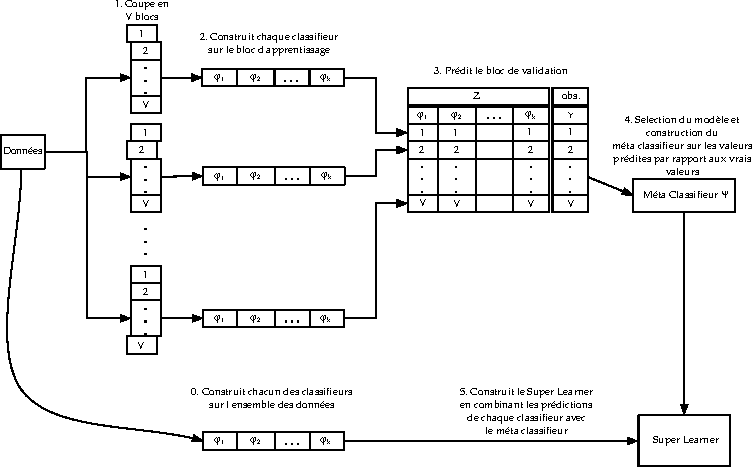
\includegraphics[scale=0.85]{../images/Superlearner.pdf}
    \caption{Fonctionnement de l'algorithme SuperLearner, adapté de \citet{VanderLaan2007a}}
\end{figure}
\end{frame}

\subsection{Combinaisons bayésiennes}

\begin{frame}
\frametitle{Combinaisons bayésiennes}
On veut prendre en compte l'incertitude quant au \textquote{vrai} modèle:
\begin{equation}
    \mathbb{P} ( \zeta \mid \mathcal{L} ) = \sum_{m=1}^M \mathbb{P} (\zeta \mid \varphi_m , \mathcal{L}) \mathbb{P} ( \varphi \mid \mathcal{L} )
    \label{equ:bma}
\end{equation} 
où $\zeta$ est une quelconque valeur d'intérêt, dans la plupart des cas $\zeta = y$ et on a donc:
\begin{equation}
    \mathbb{P} ( y_i \mid x_i , \mathcal{L} ) = \sum_{m=1}^M \mathbb{P} (y_i \mid x_i,  \varphi_m , \mathcal{L}) \mathbb{P} ( \varphi \mid \mathcal{L} )
    \label{equ:bma2}
\end{equation} 
En utilisant encore une fois le théorème de Bayes, on peut aussi écrire:
\begin{align}
    \mathbb{P} ( \varphi \mid \mathcal{L} ) &\propto \mathbb{P} ( \varphi_m ) \mathbb{P} ( \mathcal{L} \mid \varphi_m ) \\
    &\propto \mathbb{P} ( \varphi_m ) \int \mathbb{P} ( \mathcal{L} \mid \theta_m , \varphi_m ) \mathbb{P} ( \theta_m \mid \varphi_m ) \diff \theta_m
    \label{equ:bayes}
\end{align}
où $\mathbb{P} ( \theta_m \mid \varphi_m )$ est définie \emph{a priori}.
\end{frame}

\begin{frame}
\frametitle{Combinaisons bayésiennes: une correction}
Deux inconvénients majeurs mis en avant dans \citet{Minka2002}.
\begin{enumerate}
    \item L'espace d'hypothèses sur lequel on cherche la solution est nettement plus restreint que l'espace des combinaisons linéaires
    \item Tendance à converger vers le modèle le plus probable; tous les poids sont concentrés sur un unique modèle.
\end{enumerate}
Pour pallier ces $2$ problèmes, \citet{Monteith2011b} proposent une modification du BMA. Au lieu de considérer l'espace des modèles possibles $\mathcal{M}$, ils considèrent l'espace des combinaisons de $\mathcal{M}$, $C ( \mathcal{M} )$.\begin{equation}
    \mathbb{P} ( y_i \mid x_i , \mathcal{L} ) = \sum_{c \in C ( \mathcal{M} )} \mathbb{P} (y_i \mid x_i,  \varphi_m , \mathcal{L}) \mathbb{P} ( c \mid \mathcal{L} )
    \label{equ:bmc}
\end{equation}
\end{frame}

\section{Arbres et forêts}
\subsection{Arbres de classification}

\begin{frame}
\frametitle{Arbres de classification: pourquoi?}
\begin{itemize}
    \item Ils sont non-paramétriques.
    \item Ils peuvent traiter les données hétérogènes (mélange de variables qualitatives et quantitatives) ainsi que les données manquantes.
    \item Ils effectuent automatiquement une sélection des variables et sont donc en partie résistants aux variables inutiles ou bruitées.
    \item Ils sont résistants aux outliers ou erreurs d'étiquetage.
    \item Ils sont faciles d'interprétation.
\end{itemize}
\end{frame}

\begin{frame}
\frametitle{Arbres de classification: Structure}
Un \emph{arbre de décision} est un classifieur $\varphi : \mathcal{X} \rightarrow \mathcal{Y}$ représenté par un arbre enraciné où chaque nœud $t$ représente un sous-espace $\mathcal{X}_t \subseteq \mathcal{X}$ avec la racine $t_0$ représentant $\mathcal{X}$ tout entier. Les fils $t_i, \dotsc, t_j$ de $t$ représentent alors une partition disjointe de $\mathcal{X}_t$.
\begin{figure}[H]
    \centering
    \begin{subfigure}[b]{.45\textwidth}
    \centering    
    \begin{tikzpicture}
    % Draw axes
    \draw [<->,thick] (0,4) node (yaxis) [above] {$x_2$}
          |- (5,0) node (xaxis) [right] {$x_1$};
    % Draw line
    \draw[dashed] (2.7,0.1) -- (2.7,1.25);
    \draw[dashed] (2.7,1.25) -- (2.7,3.9);
    \draw[dashed] (0.1,1.35) -- (2.6,1.35);
    \draw[dashed] (1.5,0.1) -- (1.5,1.25);
    % Draw negative dots
    \fill[mDarkTeal] (0.5,1.5)   circle (3pt);
    \fill[mDarkTeal] (1.5,2.5)   circle (3pt);
    \fill[mDarkTeal] (1,2.5)     circle (3pt);
    \fill[mDarkTeal] (0.75,2)    circle (3pt);
    \fill[mDarkTeal] (0.6,1.9)   circle (3pt);
    \fill[mDarkTeal] (0.77, 2.5) circle (3pt);
    \fill[mDarkTeal] (1.5,3)     circle (3pt);
    \fill[mDarkTeal] (1.3,3.3)   circle (3pt);
    \fill[mDarkTeal] (0.6,3.2)   circle (3pt);
    \fill[mDarkTeal]   (2.2,1.2)   circle (3pt);
    \fill[mDarkTeal]   (2,1)   circle (3pt);
    \fill[mDarkTeal]   (2.3,0.7)   circle (3pt);
    % Draw positive dots
    \draw[mDarkTeal] (0.2,1.17)     circle (3pt);
    \draw[mDarkTeal] (0.5,0.2)     circle (3pt);
    \draw[mDarkTeal] (0.36,0.75)     circle (3pt);
    \draw[mDarkTeal] (0.9,0.8)     circle (3pt);
  
    \draw[mDarkTeal] (4,1)     circle (3pt); 
    \draw[mDarkTeal] (3.3,.3)  circle (3pt); 
    \draw[mDarkTeal] (4.5,1.2) circle (3pt); 
    \draw[mDarkTeal] (4.5,.5)  circle (3pt); 
    \draw[mDarkTeal] (3.9,.7)  circle (3pt); 
    \draw[mDarkTeal] (5,1)     circle (3pt); 
    \draw[mDarkTeal] (3.5,.2)  circle (3pt); 
    \draw[mDarkTeal] (4,.3)    circle (3pt); 
    \end{tikzpicture}
    \end{subfigure}
    ~
    \begin{subfigure}[b]{.45\textwidth}
    \centering
        \begin{forest}
        [$x_1 \leq 2.7$
            [$x_2 \leq 1.35$
                    [$x_1 \leq 1.5$
                        [,circle, draw]
                        [,circle, fill]
                    ]
                [,circle, fill]
            ]
            [,circle, draw]
        ]       
    \end{forest}
    \end{subfigure}
    \caption{Équivalence entre la partition du plan et un arbre de décision binaire}
\end{figure}
\end{frame}

\begin{frame}
\frametitle{Arbres de classification: minimisation de l'impureté}
\begin{definition}[Réduction de l'impureté]
    La \emph{réduction d'impureté pondérée} d'une partition binaire $s \in \mathcal{Q}$ divisant $t$ en $t_L$ et $t_R$ est:
    \begin{equation*}
        \Delta i(s,t) = i(t) - p_L i(t_L) - p_R i(t_R)
    \end{equation*}
    où $p_L$ (resp. $p_R$) est la proportion de l'échantillon dans $\mathcal{L}_t$ allant dans $t_L$ (resp. $t_R$).
\end{definition}
Notre problème de minimisation de l'\emph{impureté} est alors:
\begin{equation*}
\begin{cases}
    s^* = \operatornamewithlimits{argmax}\limits_{ \substack{s_j^* \\ j=1,\dotsc,p}} \Delta i(s^*_j,t) \\
    s^*_j = \operatornamewithlimits{argmax}\limits_{\substack{s \in \mathcal{Q}(X_j) \\ \mathcal{L}_{t_L},\mathcal{L}_{t_R} \neq \emptyset}} \Delta i(s,t)
\end{cases}
\end{equation*}
\end{frame}

\begin{frame}
\frametitle{Arbres de classification: choix de l'impureté}
\begin{theoreme}[\cite{Breiman1984a}]
\label{impurete}
    Soit $\Phi (p_1,\dotsc,p_J)$ une fonction strictement concave définie sur $0 \leq p_k \leq 1$, pour $k=1,\dotsc,J$ et $\sum_{k=1}^J p_k = 1$ telle que:
    \begin{itemize}
        \item $\Phi (1,\dotsc,0) = \Phi (0,1,\dotsc,0) = \dots = \Phi ( 0,\dotsc,1)$ soit minimale
        \item $\Phi \left(\frac{1}{J},\dotsc,\frac{1}{J} \right)$ soit maximale
    \end{itemize}
    Alors pour $i(t) := \Phi \left( p(c_1 \mid t), \dotsc, p(c_J \mid t) \right)$ et pour n'importe quel $s$,
    \begin{equation*}
        \Delta i(s,t) \geq 0
    \end{equation*}
    avec égalité si et seulement si $p(c_k \mid t_L) = p(c_k \mid t_R) = p(c_k \mid t)$ pour $k=1,\dotsc,J$.
\end{theoreme}
\end{frame}

\begin{frame}
\frametitle{Arbres de classification: exemples d'impuretés}
\begin{description}
    \item[\textbf{\textsc{Classification}}]
    \begin{align*}
        i_H (t) &= - \frac{1}{2} \sum_{k=1}^J p(c_k \mid t) \log_2 \left( p(c_k \mid t ) \right) \\
        i_G (t) &= \sum_{k=1}^J p\left(c_k \mid t \right) \left( 1-p(c_k \mid t) \right)
    \end{align*}
    \item[\textbf{\textsc{Regression}}]
    \begin{equation*}
        i_R (t) = \frac{1}{N_t} \sum_{x,y \in \mathcal{L}_t} (y-\hat{y}_t)^2
    \end{equation*}
\end{description}
\end{frame}

\subsection{Forêts aléatoires}

\begin{frame}
\frametitle{Forêts de Breiman}
\begin{itemize}
    \item Agrégation par vote majoritaire/moyenne.
    \item À chaque étape de création d'une coupure, on tire aléatoirement un sous-ensemble de $K$ variables de $\mathcal{X}$ puis on applique la procédure de choix de la coupe.
    \item Un échantillon bootstrap de l'échantillon d'apprentissage est tiré avec remise et l'arbre est construit sur ce nouvel échantillon tiré aléatoirement.
\end{itemize}

\cite{Breiman2004a} montre que la convergence des forêts aléatoires ne dépend que des variables dites \emph{fortes} et non pas des variables \emph{faibles} bruitées. Il montre que la convergence pour une version simplifiée des forêts aléatoires vers l'erreur de Bayes est de l'ordre de
\begin{equation*}
    N^{- \frac{3}{4 \vert S \vert + 3}}
\end{equation*}
avec $S$ les variables fortes définies telles que $\mathbb{E} \left[ y \mid \mathbf{x} \right]$ ne dépend que de $S$.
\end{frame}

\begin{frame}
\frametitle{Forêts de Breiman: résultats}
\begin{figure}[H]
\centering
    \begin{tikzpicture}
    \begin{axis}[domain=0:1, ymin=0, ymax = 1, enlargelimits = false, xlabel = {Taux de faux positifs}, ylabel = {Taux de vrais positifs}, legend style={draw=none,legend pos=south east, fill=none}]
            \addplot[no markers, const plot, mLightBrown] table [x = "fpr", y = "tpr", col sep = comma] {../images/roc_rf.csv};
            \addlegendentry{RF}
            \addplot[no markers] table [x = "fpr", y = "tpr", col sep = comma] {../images/roc_arbre.csv};
            \addlegendentry{CART (enveloppe)}
            \addplot[no markers, const plot, mDarkBrown] table [x = "fpr", y = "tpr", col sep = comma] {../images/roc_logreg.csv};
            \addlegendentry{LogReg}
            \addplot[no markers, black, dashed] {x};
    \end{axis}
    \end{tikzpicture}
    \caption{Performances de RF ($\mathrm{AUC} = 0.805$) par rapport à la régression logistique ($\mathrm{AUC} = 0.7889$) et un arbre seul ($\mathrm{AUC} = 0.79649$).}
\end{figure}
\end{frame}

\begin{frame}
\frametitle{Forêts obliques}
\begin{lemme}[Johnson-Lindenstrauss en distribution]
    $\forall \varepsilon > 0$, $\delta < 1/2$ et $d \in \mathbb{N}^+$ il existe une distribution $\mu$ sur $\mathcal{R}^{k \times d}$ avec $k = O( \varepsilon^{-2} \log ( 1 / \delta) )$ et $A \sim \mu$ tel que:
    \begin{equation*}
        \forall x , \Vert x \Vert = 1 : \mathbb{P} \left( \vert \Vert A x \Vert^2_2 - 1 \vert > \varepsilon \right) < \delta
    \end{equation*}
\end{lemme}
Un choix possible pour $A$ qui possède l'avantage d'accélérer grandement le produit matriciel est donné par \citet{Achlioptas2003}:
\begin{equation*}
    A_{i,j} = \sqrt{3} \begin{cases}
        +1 \text{ avec probabilité } 1/6 \\
        0 \text{ avec probabilité } 2/3 \\
        -1 \text{ avec probabilité } 1/6
    \end{cases}
\end{equation*}
\end{frame}

\begin{frame}[fragile]
\frametitle{Forêts obliques}
\begin{algorithm}[H]
\caption{Randomer Forest} \label{randomer.forest.alg}
\begin{algorithmic}
    \Procedure{Randomer Forest}{$\mathcal{L}, \mu ( \mathcal{L} )$}
    \For{chaque arbre $n$}
        \State{Création du sous-échantillon $\mathcal{L}_n$}
        \For{chaque nœud $i$ de l'arbre}
            \State{$\tilde{X}_{i,n} \gets A^\intercal_{i,n} X_n $ avec $A_{i,n} \sim \mu ( \mathcal{L}_{i,n} ) $}
            \State{$s^*_{i,n} \gets \mathrm{MeilleureCoupure} ( \tilde{X}_{i,n} )$}
            \State{Coupe $\mathcal{L}_{i,n}$ en $\mathcal{L}_{l_i,n}$ et $\mathcal{L}_{r_i,n}$ selon la règle de coupure $s^*_{i,n}$}
        \EndFor
    \EndFor
    \State \Return $\left(\mathrm{Arbres_n},\left( A_{i,n} \right) \right)$
    \EndProcedure
\end{algorithmic}    
\end{algorithm}
\end{frame}

\begin{frame}
\frametitle{Forêts bayésiennes}
\begin{itemize}
    \item On modélise les données comme une somme d'arbres.
    \item On définit un a priori sur la forme des arbres, un a priori sur les feuilles et un a priori sur l'erreur.
    \item Tirage par Bayesian Backfitting c'est-à-dire un mélange de Gibbs et Metropolis-Hastings qui exploite la forme de la somme.
\end{itemize}

Le choix des a priori est vital pour la facilité des calculs et la capacité de mélange de la chaîne de Markov: choix de lois conjuguées et chaînes réversibles quand possible.
\end{frame}

\begin{frame}
\frametitle{Forêts bayésiennes: résultats}
\begin{figure}[H]
\centering
    \begin{tikzpicture}
    \begin{axis}[domain=0:1, ymin=0, ymax = 1, enlargelimits = false, xlabel = {Taux de faux positifs}, ylabel = {Taux de vrais positifs}, legend style={draw=none,legend pos=south east,fill=none}]
            \addplot[no markers, const plot, mLightBrown] table [x = "fpr", y = "tpr", col sep = comma] {../images/roc_bart.csv};
            \addlegendentry{BART}
            \addplot[no markers, const plot] table [x = "fpr", y = "tpr", col sep = comma] {../images/roc_rf.csv};
            \addlegendentry{RF}
            \addplot[no markers, black, dashed] {x};
    \end{axis}
    \end{tikzpicture}
    \caption{Performances de BART ($\mathrm{AUC} = 0.8365$).}
\end{figure}
\end{frame}

\begin{frame}
\frametitle{Apprentissage des feuilles}
On veut séparer le processus de création de la structure d'arbre de celui d'apprentissage des étiquettes.

On peut transformer le problème d'apprentissage des feuilles pour exploiter la structure de forêt:
\begin{equation*}
\argmin_\omega \begin{cases}
        \frac{1}{N T} \sum_{i=1}^N \sum_{t=1}^T l(y_i^t , \hat{y}_i ) \\
        y_i^t = \omega_t \varphi_t (x_i ) , \forall i , t
\end{cases}
\longrightarrow
\argmin_W \begin{cases}
         \frac{1}{2} \Vert W \Vert^2_2 + \frac{C}{N} \sum_{i=1}^N l(y_i , \hat{y}_i ) \\
        y_i = W \Phi (x_i ) , \forall i
\end{cases}
\end{equation*}
On se ramène donc à un problème de SVM simple. On peut également construire une procédure d'effeuillage globale en réunissant les couples de feuilles de normes faibles.
\end{frame}

\begin{frame}
\frametitle{Apprentissage des feuilles: performances I}
\begin{figure}[H]
    \begin{tikzpicture}
    \begin{axis}[domain=0:1, ymin=0, ymax = 1, enlargelimits = false, xlabel = {Taux de faux positifs}, ylabel = {Taux de vrais positifs}, legend style={draw=none,legend pos=south east, fill=none}]
            \addplot[no markers, const plot, mLightBrown] table [x = "fpr", y = "tpr", col sep = comma] {../images/roc_erf.csv};
            \addlegendentry{ERF}
            \addplot[no markers, const plot] table [x = "fpr", y = "tpr", col sep = comma] {../images/roc_rf.csv};
            \addlegendentry{RF}
            \addplot[no markers, black, dashed] {x};
    \end{axis}
    \end{tikzpicture}
    \caption{Performances de ERF ($\mathrm{AUC} = 0.7664$).}
\end{figure}
\end{frame}

\begin{frame}
\frametitle{Apprentissage des feuilles: optimisation de l'AUC}
On peut aussi chercher à apprendre les feuilles de façon à optimiser l'AUC.
\begin{equation*}
    \mathrm{AUC} ( \varphi , \mathcal{L} ) = \frac{\sum_{k_0 \in \mathcal{L_0}} \sum_{k_1 \in \mathcal{L_1}} \mathds{1}_{\varphi(x_0) < \varphi(x_1)} }{\vert \mathcal{L}_0 \vert \vert \mathcal{L}_1 \vert }
\end{equation*}
Mais l'AUC n'est pas dérivable. On va alors optimiser un substitut:
\begin{equation*}
    \mathrm{AUC} ( \varphi , \mathcal{L} ) = \frac{\sum_{k_0 \in \mathcal{L_0}} \sum_{k_1 \in \mathcal{L_1}} f \left( \varphi(x_1) - \varphi(x_0) \right) }{\vert \mathcal{L}_0 \vert \vert \mathcal{L}_1 \vert }
\end{equation*}
avec $f$ dérivable.
\end{frame}

%\begin{frame}
%\frametitle{Apprentissage des feuilles: optimisation de l'AUC}
%Bien que cela suffise en théorie pour optimiser l'AUC il faut en pratique recalculer l'AUC à chaque étape de l'optimisation, et le coût de celui-ci est quadratique.
%On peut montrer qu'optimiser une approximation de l'AUC où l'on a remplacé $f$ par une approximation polynomiale de $f$ permet de faire apparaître un certain nombre de quantités que l'on peut calculer une unique fois. On se ramène ainsi au cas linéaire.
%\end{frame}

\section{Données déséquilibrées}

\begin{frame}
\frametitle{Forêts aléatoires équilibrées}
Le sous-échantillonnage permet d'éviter le sur-apprentissage de la classe majoritaire et implicitement l'attribution de poids plus importants à la classe majoritaire. De plus le sous-échantillonnage a pour effet secondaire d'accélérer l'apprentissage.
\begin{itemize}
    \item On peut effectuer un sous-échantillonnage directement durant l'étape bootstrap en forçant l'équilibre.
    \item On peut également équilibrer \textquote{en moyenne} afin de diminuer encore plus la corrélation entre les arbres tout en gardant un certain équilibre.
    \item La proportion optimale n'est pas forcément 50/50. On peut donc également effectuer un sous-échantillonnage non équilibré. (Proportion $\frac{1}{2} + \frac{2 q_a - 1}{4}$)
\end{itemize}
\end{frame}

\begin{frame}
\frametitle{Forêts aléatoires équilibrées: performances}
    \begin{figure}[H]
    \centering
    \begin{tikzpicture}
    \begin{axis}[name= plot1, width=0.5\textwidth, domain=0:1, ymin=0, ymax = 1, enlargelimits = false, xlabel = {Taux de faux positifs}, ylabel = {Taux de vrais positifs}, legend style={draw=none,legend pos=south east, fill=none}]
            \addplot[no markers, const plot, mLightBrown] table [x = "fpr", y = "tpr", col sep = comma] {../images/roc_nbrf.csv};
            \addlegendentry{NBRF}
            \addplot[no markers, const plot, mDarkBrown] table [x = "fpr", y = "tpr", col sep = comma] {../images/roc_brf.csv};
            \addlegendentry{BRF}
            \addplot[no markers, const plot] table [x = "fpr", y = "tpr", col sep = comma] {../images/roc_rf.csv};
            \addlegendentry{RF}
            \addplot[no markers, black, dashed] {x};
    \end{axis}

    \begin{axis}[name = plot2, width=0.5\textwidth, at=(plot1.right of south east), anchor=left of south west, domain=0:1, ymin=0, ymax = 1, enlargelimits = false, xlabel = {Taux de faux positifs}, legend style={draw=none,legend pos=south east, fill=none}]
            \addplot[no markers, const plot, mLightBrown] table [x = "fpr", y = "tpr", col sep = comma] {../images/roc_vrbrf.csv};
            \addlegendentry{VRBRF}
            \addplot[no markers, const plot, mDarkBrown] table [x = "fpr", y = "tpr", col sep = comma] {../images/roc_rbrf.csv};
            \addlegendentry{RBRF}
            \addplot[no markers, const plot] table [x = "fpr", y = "tpr", col sep = comma] {../images/roc_rf.csv};
            \addlegendentry{RF}
            \addplot[no markers, black, dashed] {x};
    \end{axis}
    \end{tikzpicture}
    \caption{Performances de BRF ($\mathrm{AUC} = 0.8432$), NBRF ($\mathrm{AUC} = 0.8427$), RBRF ($\mathrm{AUC} = 0.8432$) et VRBRF ($\mathrm{AUC} = 0.8421$)}
\end{figure}
\end{frame}

\begin{frame}
\frametitle{Meta-Cost}
Puisque les classes majoritaires et minoritaires n'ont pas la même importance, on introduit un coût de mauvaise classification. On cherche alors à minimiser le risque conditionnel 
\begin{equation}
    R ( i \mid x ) = \sum_j \mathbb{P} ( j \mid x ) C(i,j) \label{idee_metacost}
\end{equation}
On peut alors:
\begin{enumerate}
    \item Utiliser notre classifieur pour déterminer la probabilité inconnue (par bagging par exemple si le classifieur ne donne pas de probabilité naturellement).
    \item Résoudre l'équation~\ref{idee_metacost}
    \item Remplacer dans l'échantillon les vraies étiquettes par les étiquettes \textquote{idéales} trouvées précédemment.
    \item Apprendre notre classifieur final sur ce nouvel échantillon.
\end{enumerate}
\end{frame}

\begin{frame}[fragile]
\begin{algorithm}[H]
\caption{Algorithme Metacost pour les forêts aléatoires}\label{alg:metacost}
\begin{algorithmic}
    \Procedure{Metacost-RF}{$S, C$}
    
    \State{ \texttt{RF} $\gets$ \texttt{ForêtsAléatoire(S)} }
    
    \For{ $(y,x) \in S$ }
        \For{ chaque classe $j$ }
            \If{$x \in \operatorname{OOB}(\texttt{RF})$}
                \State{ $\hat{p}(j \mid x) \gets \mathbb{P}_{\text{OOB}}(j \mid x)$ }
            \Else \State{$\hat{p}(j \mid x) \gets \texttt{RF}(j \mid x)$}
            \EndIf
        \EndFor
        \State{$y \gets \argmin_i \sum_j \hat{p}(j \mid x) C(i,j)$}
    \EndFor
    \State \Return $S$
    \EndProcedure
\end{algorithmic}    
\end{algorithm}
\end{frame}


\begin{frame}
\frametitle{Meta-Cost: performances}
\begin{figure}[H]
\centering
    \begin{tikzpicture}
    \begin{axis}[domain=0:1, ymin=0, ymax = 1, enlargelimits = false, xlabel = {Taux de faux positifs}, ylabel = {Taux de vrais positifs}, legend style={draw=none,legend pos=south east, fill=none}]
            \addplot[no markers, const plot,mLightBrown] table [x = "fpr", y = "tpr", col sep = comma] {../images/roc_mcrf.csv};
            \addlegendentry{RF+MC}
            \addplot[no markers, const plot] table [x = "fpr", y = "tpr", col sep = comma] {../images/roc_rf.csv};
            \addlegendentry{RF}
            \addplot[no markers, black, dashed] {x};
    \end{axis}
    \end{tikzpicture}
    \caption{Performances de MetaCost + RF ($\mathrm{AUC} = 0.8217$).}
\end{figure}
\end{frame}

\section{Résultats}

\begin{frame}
\frametitle{Résultats}
\vspace{-1.1cm}
\small{
\begin{table}[H]
    \centering
    \begin{tabular}{lrrrr}
    \toprule
    & \multicolumn{2}{c}{Base A}  & \multicolumn{2}{c}{Base B} \\ 
    \cmidrule(lr){2-3} \cmidrule(lr){4-5}
    Classifieur & AUC & Brier & AUC & Brier \\
    \midrule
    Régression logistique & $0.789$ & $0.031$ & $0.673$ & $0.024$ \\
    CART & $0.796$ & $0.032$ & $0.654$ & $0.025$ \\
    Forêts aléatoires & $0.805$ & $0.029$ & $0.699$ & $0.023$ \\
    Boosting Arbres & $0.810$ & $0.030$ & $0.635$ & $0.025$ \\
    %Stacking $\sim$ Linéaire & & & & \\
    %Stacking $\sim$ Logistique & & & & \\
    Stacking $\sim$ Réseau de neurones & $0.737$ & $0.040$ & $0.632$ & $0.025$ \\
    Balanced RF & $0.843$ & $0.151$ & $0.717$ & $0.145$ \\
    Weighted RF & $0.801$ & $0.029$ & $0.702$ & $0.023$ \\
    Roughly Balanced RF & $0.843$ & $0.154$ & $0.721$ & $0.146$ \\
    Nearly Balanced RF & $0.843$ & $0.133$ & $0.724$ & $0.122$ \\
    Very Roughly Balanced RF & $0.842$ & $0.130$ & $0.721$ & $0.121$ \\
    RF + Metacost & $0.822$ & $0.294$ & $0.698$ & $0.189$ \\
    RF + Feuilles SVMs & $0.766$ & $0.114$ & $0.590$ & $0.025$ \\
    RF Uniformes & $0.842$ & $0.028$ & $0.705$ & $0.024$ \\
    RF Uniformes Équilibrées & $0.843$ & $0.215$ & $0.731$ & $0.208$ \\
    ExtRa-Trees & $0.779$ & $0.029$ & $0.675$ & $0.025$ \\
    BART & $0.837$ & $0.027$ & $0.732$ & $0.023$ \\
    \bottomrule
    \end{tabular}
    \caption{Performances des différentes méthodes sur $2$ bases de validation différentes}\label{table:resultats}
\end{table}
}
\end{frame}

\plain{Conclusion}

\begin{frame}
\frametitle{Conclusion}
\begin{itemize}
    \item Méthodes ensemblistes: façon simple d'améliorer les performances.
    \item Rééquilibrage crucial.
    \item Très bonnes performances prédictives des méthodes bayésiennes, très mauvaises performances computationnelles: perspectives d'amélioration intéressantes.
    \item Il semble judicieux de se concentrer sur les méthodes de \emph{ranking} et d'optimiser l'AUC directement au lieu de réadapter les méthodes d'apprentissage classiques.
\end{itemize}
\end{frame}

\plain{Merci}

\section*{Annexe}

\begin{frame}
\frametitle{Metropolis-Hastings: I}
Condition suffisante (non nécessaire) pour assurer que $p(\theta)$ est la distribution invariante est la condition de réversibilité:
\begin{equation}\label{equ:detailed.balance}
    p( \theta_i ) g ( \theta_{i-1} \mid \theta_i ) = p( \theta_{i-1} ) g ( \theta_{i} \mid \theta_{i-1} )
\end{equation}

L'algorithme de Metropolis-Hastings utilise alors une densité de proposition $q (\theta' \mid \theta)$, qui joue le rôle de chaîne de Markov continue. À partir de $\theta$, une valeur $\theta'$ est proposée puis acceptée comme nouvel état avec probabilité:
\begin{equation*}
    A(\theta,\theta') = \min \left\{ 1 , \frac{p(\theta') q(\theta \mid \theta')}{p(\theta) q(\theta'\mid \theta} \right\}
\end{equation*}
\end{frame}

\begin{frame}
\frametitle{Théorème ergodique}
\begin{theoreme}[Théorème Ergodique]\label{thrm:ergodique}
    Soient $\hat{\theta}_1,\dotsc,\hat{\theta}_m$ une suite de valeurs d'une chaîne de Markov de noyaux de transition $g$, et matrice de transition $P$, telle que la chaîne soit:
    \begin{align*}
                &\exists i , \forall j > i,  g \left( \hat{\theta}_j \mid \hat{\theta}_i \right) > 0 \\
                &\forall i,j \; g \left( \hat{\theta}_j \mid \hat{\theta}_j \right) > 0 \\
            &\forall i , \mathbb{E} \left[ T_i \right] < \infty \\
            &T_i = \inf \left\{ j \geq 1 : \hat{\theta}_j = i \mid \hat{\theta}_0 = i \right\}
    \end{align*}
    Alors si $\mathbb{E} \left[ f(\theta) \right] < \infty$ alors
    \begin{equation*}
        \mathbb{P} \left( \frac{1}{n} \sum_{i=1}^n f(\hat{\theta}_i) \to \int f(\theta) \pi ( \theta ) \diff \theta \right)
    \end{equation*}
    où $\pi$ est la distribution stationnaire de la chaîne de Markov c'est-à-dire $\pi = \pi P$
\end{theoreme}
\end{frame}

\begin{frame}[fragile]
\frametitle{Metropolis-Hastings: II}
\begin{algorithm}[H]
\caption{Metropolis-Hastings} \label{metropolis.hastings.alg}
\begin{algorithmic}
    \Procedure{Metropolis-Hastings}{$q, \theta_0, n$}
    \For{$i \in [0,n-1] $}
        \State{Tire $u \sim \mathcal{U}_{[0,1]} $}
        \State{Tire $\theta' \sim q(\theta' \mid \theta_i)$}
        \If{$u < \min \left\{ 1 , \frac{p(\theta') q(\theta_i \mid \theta')}{p(\theta_i) q(\theta'\mid \theta_i)} \right\}$}
            \State{$\theta_{i+1} = \theta'$}
        \Else \State{$\theta_{i+1} = \theta_i$}
        \EndIf
    \EndFor
    \State \Return $(\theta_0,\cdots,\theta_{n-1})$
    \EndProcedure
\end{algorithmic}
\end{algorithm}
\end{frame}

\begin{frame}
\frametitle{Metropolis-Hastings: III}
On a ici que
\begin{equation*}
    g( \theta_i , \theta_{i+1} ) = q ( \theta_{i+1} \mid \theta_{i} ) A(\theta_{i},\theta_{i+1}) + \delta_{\theta_{i}} ( \theta_{i+1} ) R(\theta_{i})
\end{equation*}
Avec $R\theta_{i}$ le terme de rejet:
\begin{equation*}
    R(\theta_{i}) = \int q ( \theta \mid \theta_{i} ) ( 1 - A(\theta_{i},\theta) ) \diff \theta
\end{equation*}
Par construction $g$ remplis la propriété~\ref{equ:detailed.balance}. De plus, le terme de rejet garantit l'apériodicité et il suffit que le support de $q$ inclue le support de $p$ pour garantir l'irréductibilité.

La présence de $p$ non seulement au numérateur, mais aussi au dénominateur permet de se débarrasser de la constante de renormalisation, souvent l'un des éléments les plus contraignants.
\end{frame}

\begin{frame}[fragile]
\frametitle{Problèmes avec l'approximation de l'AUC}
\begin{figure}[H]
    \centering
    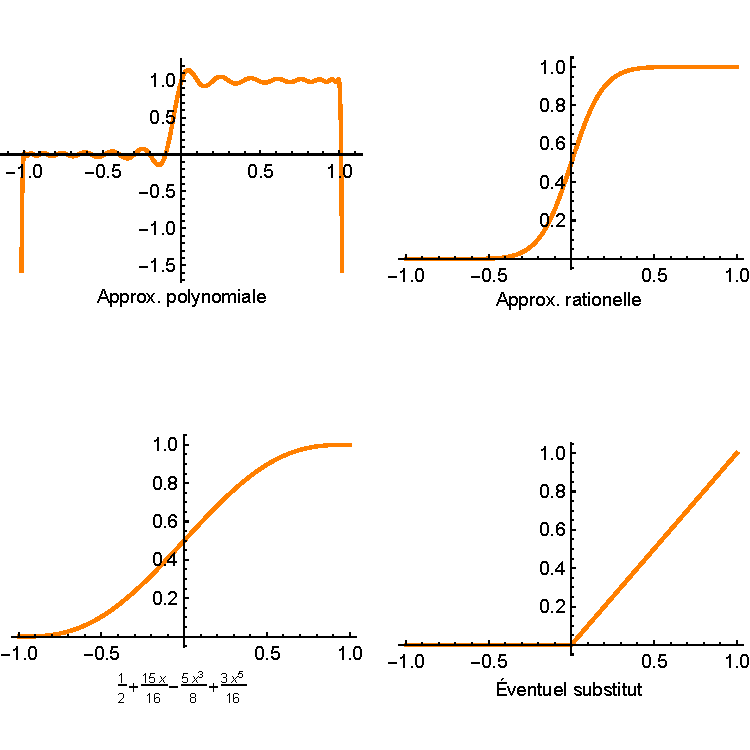
\includegraphics[scale=0.6]{../images/graphs2}
\end{figure}
\end{frame}

\end{document}